\chapter{Perancangan}
\label{chap:perancangan}

Pada bab ini akan dijelaskan perancangan mengenai simulator yang akan dibangun untuk pertumbuhan wirausaha. Perancangan yang dibuat akan meliputi diagram kelas beserta penjelasannya dan rancangan antarmuka dari perangkat lunak.


\section{Diagram Kelas}
\label{sec:perancangankelas}

Dalam membuat simulator diperlukan sebuah GUI atau Interface untuk bisa menggambarkan kinerja suatu sistem. Berdasarkan hasil pengembangan diagram kelas pada bab analisis \ref{fig:CD1}, dibuatlah diagram kelas rinci untuk memenuhi kebutuhan dalam membangun simulator. Deskripsi kelas beserta fungsinya akan dijelaskan pada subbab selanjutnya.

\begin{figure} [H]
	\centering  
	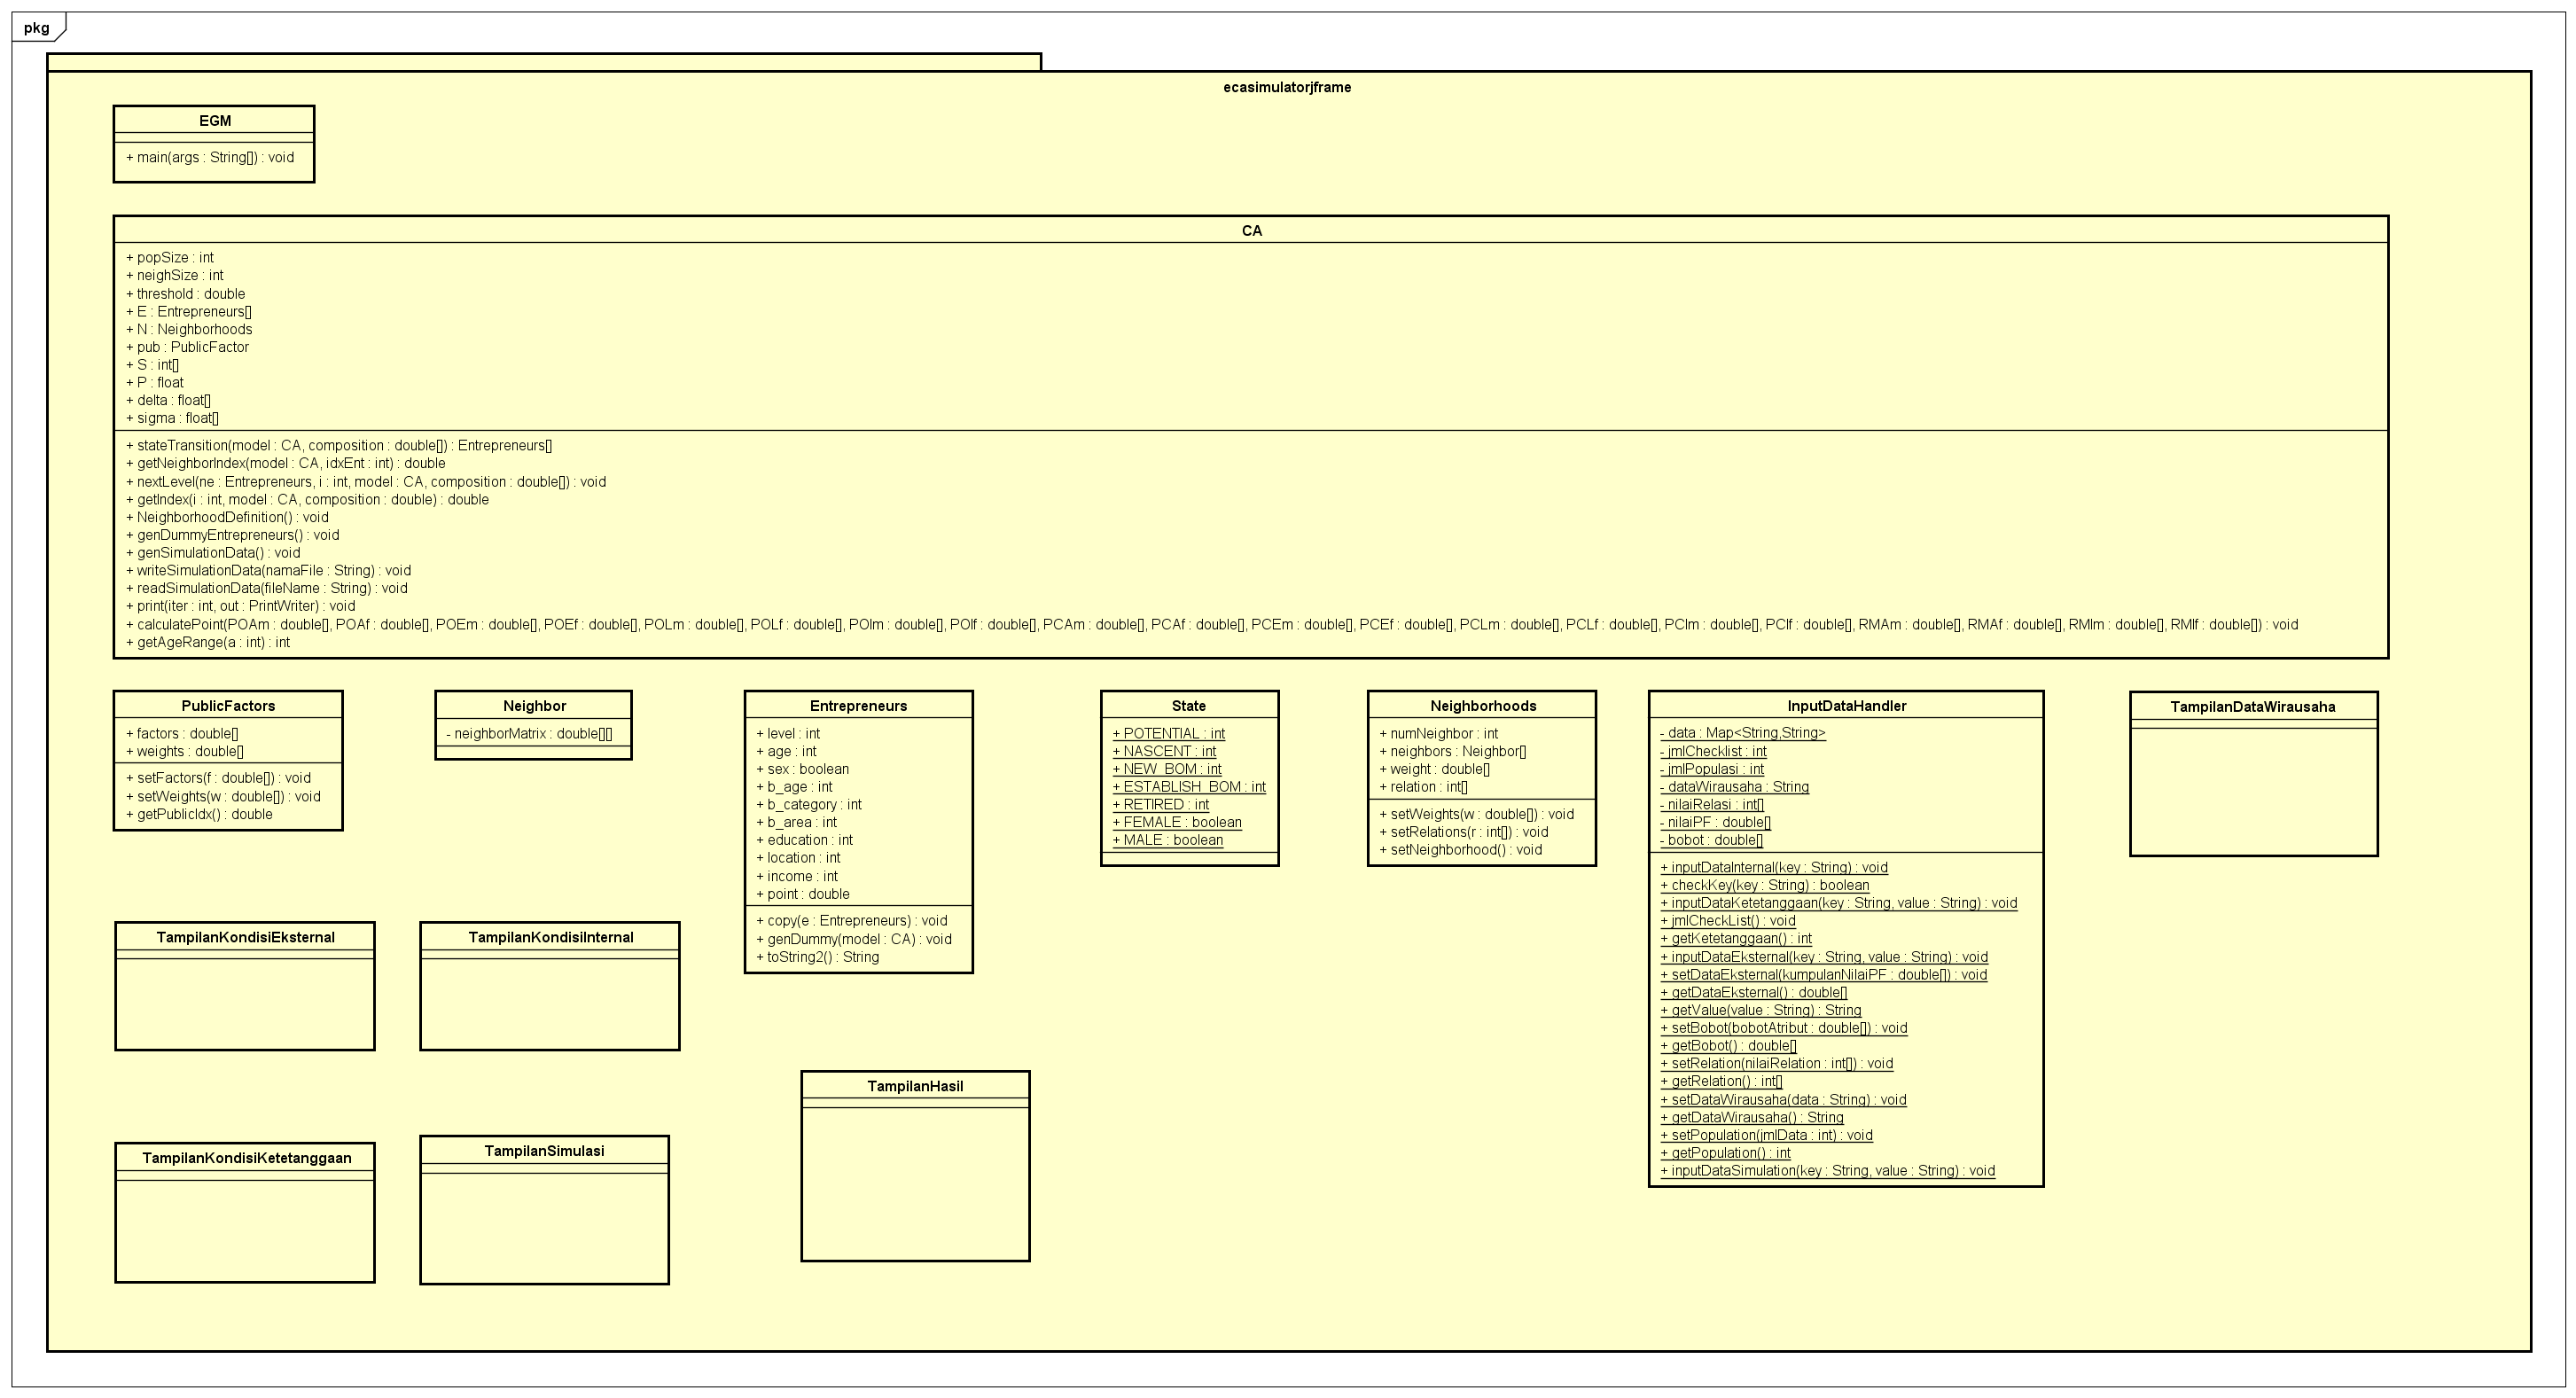
\includegraphics[width=18cm, height=12cm]{ClassDiagram3} 
	\label{fig:classdiagram2} 
\end{figure}


\subsection{Kelas TampilanKondisiInternal}
Kelas ini merupakan kelas untuk menampilkan seluruh atribut umum dari seorang wirausaha yang dapat dipilih menggunakan \textit{checkbox}, atribut yang dipilih nantinya akan mempengaruhi ketetanggaan antara wirausaha yang satu dengan wirausaha lainnya. Setelah itu, \textit{user} diminta mengisi bobot untuk masing-masing atribut yang sudah dichecklist melalui \textit{textfield}.

\subsection{Kelas TampilanKondisiKetetanggaan}
Kelas ini merupakan kelas untuk menampilkan atribut yang sudah dipilih dari kelas TampilanKondisiInternal. \textit{User} dapat memilih atribut mana saja yang akan ditetapkan menjadi kondisi ketetanggaan untuk satu wirausaha ke wirausaha lainnya. Selain itu, \textit{user} diminta untuk mengisi hubungan ketetanggaan khusus untuk 4 atribut yaitu umur, level, pendapatan dan pendidikan jika \textit{user} men-checklist salah satu atau bahkan keempat-empatnya dari atribut tersebut. Untuk atribut jenis kelamin, lokasi usaha dan bidang usaha tidak dapat ditetapkan menjadi 3 jenis karena jenisnya hanya satu yaitu sama dengan. Alasan ketiga atribut tersebut tidak bisa ditetapkan menjadi 3 jenis karena ketiga atribut tersebut tidak bisa diurutkan atau dibandingkan seperti atribut a lebih besar dari atribut b.

\subsection{Kelas TampilanKondisiEksternal}
Kelas ini merupakan kelas untuk menampilkan faktor eksternal yang mempengaruhi pertumbuhan wirausaha. Dalam kasus ini ditetapkan 4 faktor saja yaitu program pemerintah, dinamika pasar, norma,sosial dan budaya, serta infrastruktur fisik dan akses layanan. \textit{User} diminta untuk mengisi bobot untuk setiap faktor dan total dari semua bobot harus 100\%.

\subsection{Kelas DataWirausaha}
Kelas ini merupakan kelas untuk membuka file data wirausaha dan menampilkannya ke tabel.

\subsection{Kelas TampilanSimulasi}
Kelas ini untuk menghitung CIDx.
\subsection{Kelas InputDataHandler}
Kelas ini merupakan kelas untuk mengambil dan menyimpan data masukan dari \textit{user}. 